\documentclass[xcolor=dvipsnames]{beamer}
\mode<presentation>

%% This is the original
%%\usetheme[secheader]{myBoadilla2}

\usetheme{myFrankfurt}
%\usetheme{Darmstadt}
%\useoutertheme{miniframes}
\useoutertheme[subsection=false]{mysmoothbars}
%\usecolortheme{crane}
\usecolortheme{wolverine}

\makeatletter
  \beamer@compressfalse
\makeatother
%% Issues with multiple lines, etc for dots
% http://tex.stackexchange.com/questions/35796/how-can-i-get-multiple-lines-of-frame-dots-in-beamer-navigation

%\useoutertheme[subsection=false]{mysmoothbars}

%% \useoutertheme{shadow} %% the one used often by Dirk


\setbeamertemplate{itemize item}[ball]
%\usetheme[left]{Goettingen}
%\usetheme[left,hideothersubsections]{myGoettingen}
%\usepackage{CSIC2}
\setbeamertemplate{itemize item}[ball]


 \setbeamertemplate{navigation symbols}{
%% I do not use or need them
 %%     \insertslidenavigationsymbol
 }


%\usepackage{Sweave} 
\usepackage[absolute,overlay]{textpos}
%\usepackage[spanish]{babel} % can do funny things with \lim \min
\usepackage[english]{babel}
\usepackage[latin1]{inputenc}
\usepackage{times}
\usepackage[T1]{fontenc}
% Or whatever. Note that the encoding and the font should match. If T1
% does not look nice, try deleting the line with the fontenc.
%%\usepackage{fancybox}

\usepackage{url}
\definecolor{light-gray}{gray}{0.72}

\newcommand{\cyan}[1]{{\textcolor {cyan} {#1}}}
\newcommand{\blu}[1]{{\textcolor {blue} {#1}}}
\newcommand{\Burl}[1]{\blu{\url{#1}}}
\newcommand{\red}[1]{{\textcolor {red} {#1}}}
\newcommand{\green}[1]{{\textcolor {green} {#1}}}
\newcommand{\mg}[1]{{\textcolor {magenta} {#1}}}
\newcommand{\og}[1]{{\textcolor {PineGreen} {#1}}}
\newcommand{\code}[1]{\texttt{\slshape\footnotesize #1}}
\newcommand{\myverb}[1]{{\footnotesize\texttt {\textbf{#1}}}}
\newcommand{\Rnl}{\ +\qquad\ }
\newcommand{\Emph}[1]{\emph{\mg{#1}}}

\usepackage{gitinfo2}

\newcommand{\hanging}[1]{ 
\renewcommand{\baselinestretch}{0.7}\small\normalsize
\setlength{\parskip}{1.5ex plus0ex minus0ex}
  \noindent\hangindent=24pt
  \hangafter=1 
   {\scriptsize #1}
  %\hangindent\parindent
}   


\newcommand{\hango}[1]{ 
\renewcommand{\baselinestretch}{0.7}\small\normalsize
\setlength{\parskip}{1.5ex plus0ex minus0ex}
  \noindent\hangindent=24pt
  \hangafter=1 
   {\tiny #1}
  %\hangindent\parindent
}   


\newcommand{\hanginp}[2]{ 
  \renewcommand{\baselinestretch}{0.7}\small\normalsize
  \setlength{\parskip}{1.5ex plus0ex minus0ex}
  \noindent\hangindent=24pt
  \hangafter=1 
  {\scriptsize #1}{\hspace{2pt}\Large\red{#2}}
  % \hangindent\parindent
}   


%% use for itemize wihtin description
% \newenvironment{myitemize} {
%   \setlength{\leftmarginii}{-10mm}
%   \itemize
% }

% \newenvironment{myitemize}
% {\setlength{\leftmarginii}{-10mm}
% \begin{itemize}}
% {\end{itemize}}


\newenvironment{myitemize}
{\begin{itemize}}{\end{itemize}}


\newcommand{\mydes}[2][]{
  \vspace*{-1pt}
%%  \renewcommand{\baselinestretch}{0.7}\small\normalsize
  \begin{description}\item[{#2}]{#1}\end{description}
\vspace*{-8pt}
}


%% what follows is a mess.
%% with R-2.12 I used es_ES. With 2.14, I comment that out.



\usepackage{tikz}
\usetikzlibrary{arrows,shapes,positioning,backgrounds}

\tikzset{
  % Define standard arrow tip
  >=stealth',
  % Define style for boxes
  punkt/.style={
    rectangle,
    rounded corners,
    draw=black, very thick,
    %maximum width=6em,
    %text width=6.5em,
    minimum height=2em,
    text centered},
  punkk/.style={
    rectangle,
    rounded corners=3mm,
    draw=black, very thick,
    %text width=6.5em,
    minimum height=2em,
    text centered},
  punkr/.style={
    rectangle,
    draw=black, very thick,
    %maximum width=6em,
    %text width=6.5em,
    minimum height=2em,
    text centered},
  punkr2/.style={
    rectangle,
    draw=black, very thick,
    inner sep = 4pt,
    %maximum width=6em,
    %text width=6.5em,
    %minimum height=2em,
    text centered},
 punkk2/.style={
    rectangle,
    rounded corners=3mm,
    draw=black, very thick,
    inner sep = 4pt,
    %text width=6.5em,
    %minimum height=2em,
    text centered},
  % Define arrow style
  pil/.style={
    ->,
    thick,
    shorten <=2pt,
    shorten >=2pt,}
}




\title[Intro to the course] {BM-13: Bioinform�tica Avanzada y Biolog�a de Sistemas, 2014-2015\\ 
Introduction to the course}

% \subtitle
% {Review and reflections} % (optional)

\author[]{Ram�n D�az-Uriarte} %% \\ \Burl{http://ligarto.org/rdiaz}}

\institute[]{Dept. Bioqu�mica\\
Universidad Aut�noma de Madrid\\
Madrid, Spain\\
\texttt{rdiaz02@gmail.com}\\
\Burl{http://ligarto.org/rdiaz}
}



\date{\gitAuthorDate\ {\footnotesize (Release\gitRels: Rev:
    \gitAbbrevHash)}}


\begin{document}



\begin{frame}
  \titlepage
\end{frame}



\begin{frame} 
\frametitle{License and copyright}

\begin{center}

\includegraphics[%
     width=3.2cm,
     keepaspectratio]
{by-sa.eps}
\vspace{10pt}

{\footnotesize This work is Copyright, \copyright, 2014, Ramon Diaz-Uriarte, and is
licensed under the \textbf{Creative Commons }
Attribution-ShareAlike 4.0 International License:
\Burl{http://creativecommons.org/licenses/by-sa/4.0/}.
}
\end{center}
\centerline{*****************************} {\scriptsize Please,
  \textbf{respect the copyright and license}. This material is provided
  freely. If you use it, I only ask that you use it according to the (very
  permissive) terms of the license: acknowledging the author, and
  redistributing copies and derivatives under the same license. If you
  have any doubts, ask me.}

\vspace{5pt}
{\tiny All of the original \LaTeX\ files are available from github:
  \Burl{https://github.com/rdiaz02/BM-13}}
\end{frame}



% \begin{frame} 
% \frametitle{License and copyright}

% \begin{center}

% \includegraphics[%
%      width=5.2cm,
%      keepaspectratio]
% {cc-by-nc-sa-eu.pdf}
% \vspace{15pt}

% This work is Copyright, \copyright, 2011, Ram�n D�az-Uriarte, and is 
% licensed under the \textbf{Creative Commons }
% Attribution-NonCommercial-ShareAlike License. 
% To view a copy of this license, visit\\ 
% \Burl{http://creativecommons.org/licenses/by-nc-sa/3.0/} 
% or send a letter to Creative Commons, 
% 559 Nathan Abbott Way, Stanford, California 94305, USA.

% \end{center}
% \centerline{*****************************}
% {\scriptsize Please, \textbf{respect the copyright}. This material is provided freely,
% and if you use it, I only ask that you use it according to the (very
% permissive) terms of the license: attribution, non-comercial use, and a share
% alike license. If you have any doubts, ask me.}

% \end{frame}





 \begin{frame}
   \frametitle{Outline}
 {\small
 \tableofcontents[subsectionstyle=hide]
 }
 \end{frame}

\section{Skills, topics}
\subsection{} %% to get the dots in header
%% a know issue https://bitbucket.org/rivanvx/beamer/issue/218/miniframes-and-smoothbars-dont-show

\begin{frame}
\frametitle{Objectives: skills and attitudes}
\begin{itemize}
\item Acquire skills and attitudes
  \begin{itemize}
  \item Get used to reading and \textbf{working through} the primary literature
  \end{itemize}
\end{itemize}
\end{frame}


\begin{frame}
  \frametitle{What will be covered?}
  \begin{itemize}
  \item Just a few things.
  \item We can argue all/most/many of them are of fundamental importance.
  \item Some are covered because of their general applicability and/or
    because they show a way of thinking about, and solving, problems.
  \end{itemize}
\end{frame}



\begin{frame}
  \frametitle{What will not be covered?}
  \begin{itemize}
  \item If we only cover a few things \ldots 
  \item we will not cover most of what falls under ``Bioinformatics''.

\pause
\vspace*{15pt}
\item Protein prediction and folding.
\item RNA prediction.
\item Sequencing (NGS and all that).
\item aCGH.
\item \ldots
  \end{itemize}
\end{frame}



\begin{frame}
  \frametitle{What and how?}

\begin{tikzpicture}[node distance=1cm, auto,]
\path[use as bounding box] (-2,-1.9);  %-2, -2.6
 %nodes
\onslide+<1-> {

 \node[punkt,text width=2cm] (bd) {Portals and databases};
 \node[right=of bd,xshift=5mm,punkt] (tools) {Tools};
 \draw[-] (tools) to (bd);

 \node[below=of tools,xshift=0mm,yshift=5mm,punkk] (methods) {Methods};
 \node[right=of methods,punkk] (razon) {Reasonings};

 \draw[<-] (tools) to (methods);
% \draw[<-] (tools) to (razon);
 \draw[<-] (methods) to (razon);

 \node[below=of methods,xshift=-13mm,yshift=5mm,punkk] (algo) {Algorithms};
 \node[below=of methods,xshift=13mm,yshift=5mm,punkk] (stats) {Statistics};
% \node[below=of razon,punkk,yshift=5mm,text width=2cm] (filog) {Evoluci�n/ Filogenia};

 \draw[-] (methods) to (algo);
 \draw[-] (methods) to (stats);
% \draw[-] (razon) to (filog);

 % \node [xshift=-0.86cm,yshift=-7.35cm] at (current page.south west)  {\scriptsize[Secci�n \ref{D-bbms-objetivos-detalles}, p.\ \pageref{D-bbms-objetivos-detalles}]};


}


{\footnotesize

 \onslide+<2-> {
\node[below=of stats,yshift=-2mm,xshift=2mm,text width=1.82cm,punkk]
(criteria) {Develop criteria};
 \node[left=of criteria,punkk,xshift=5mm,text width=2.4cm] (man)
 {Documentation, manuals, literature} 
 edge [->] (criteria); 

 \node[left=of man,punkk,text width=1.5cm,xshift=5mm] (info) {Search for info}
edge [<-] (man);

 % \node[below=of man,punkk,text width=1.7cm]
 % (act) {Actitudes/ Aptitudes}
 % edge[->] (criteria)
 % edge[->] (info);
 
 % \onslide+<4->\draw[-] (act) to (criteria);
 % \onslide+<4->\draw[-] (act) to (info);

 \draw[.,bend left,color=light-gray] (info) to (bd);
 \draw[.,color=light-gray] (criteria) to (algo);
 \draw[.,color=light-gray] (criteria) to (stats);
 \draw[.,color=light-gray] (criteria) to (razon);

}
}


% \onslide+<3-> {

% }
\end{tikzpicture}
\end{frame}



\begin{frame}
  \frametitle{What and how}
  \begin{itemize}
  \item A few key topics.
  \item Solutions ``by hand''.
  \item Very little computer use.
  \item Read the literature. 
  \end{itemize}
\end{frame}



\begin{frame}
  \frametitle{Some references to the underlying philosophy}
  \begin{itemize}
  \item See papers in Moodle if you are curious
  \item Durbin et al., and a couple from Pevzner and others.
  \end{itemize}
\end{frame}


\section{Schedule and organization}
\subsection{} %% to get the dots in header


\begin{frame}
  \frametitle{Moodle}
  \begin{itemize}
  \item \Burl{https://moodle.uam.es/course/view.php?id=9285}
  \item In UAM's Moodle, it is course ``2014\_31045\_150\_1'' or
    ``BM-13-meta''
  \item (your group does not matter; this should be a ``meta course'')
  \end{itemize}
\end{frame}


\begin{frame}
  \frametitle{Moodle}
  \begin{itemize}
  \item \textbf{ALL} of you should use that course.
  \item (If you see other BM-13s in moodle they will NOT be used).
  \item We might do the final exam in Moodle.
  \end{itemize}
\end{frame}


\begin{frame}
  \frametitle{Course material}
  \begin{itemize}
  \item In Moodle
  \item All of my original \LaTeX\ files are publicly available from
    github: \Burl{https://github.com/rdiaz02/BM-13}
  \end{itemize}
\end{frame}



\begin{frame}
  \frametitle{Grading}
  \begin{itemize}
  \item Grading: guia docente.
  \item Exercises: hand them to me when we are done with each block.
  \item Final exam: in class, multiple choice.
  \item (If you try hard enough) You can fail this course.
  \end{itemize}
\end{frame}


\begin{frame}
  \frametitle{Schedule and organization}
  \begin{itemize}
  \item Go to schedule.
  \item Class duration: 3 * 50 with 5 min.\ break?
%%  \item Grading: guia docente.
  \item Exercises: hand them to me when we are done with each block:
    \begin{itemize}
    \item the  first day of the following block.
    \end{itemize}

  \item Classes: what we will do in class. 
    \begin{itemize}
    \item Bloques 2, 3, 5, 6: no lectures as such. {\scriptsize But I'll
        do a short intro. \textbf{You MUST} read the material before class.}
    \end{itemize}
  \item How many of you have looked at the notes? %% Exercises? 
  \end{itemize}
\end{frame}




% \begin{frame}
% \frametitle{Este curso se puede suspender}
% \begin{itemize}
% \item (If you try hard enough) You can fail this course
% \end{itemize}
% \end{frame}



\begin{frame}
  \frametitle{Bologna}
  \begin{itemize}
  \item Why?
    \begin{itemize}
    \item We have to (it is the law)
    \item It might even be good:
      \begin{itemize}
      \item Learn how to learn on your own
      \item Active learning: better retention
      \item Focus on what is difficult
      \item (It is a \textbf{lot} more work)
%% Para mi es: preparar con antelacion, mucho m�s expuesto, y corregir
%% deberes A MANO!!!
      \end{itemize}
    \end{itemize}
  \item How?
    \begin{itemize}
    \item Not unlike BM-1 but \ldots
      \begin{itemize}
      \item Read the material
      \item Really: \textbf{do read the material}
      \item Do exercises
      \end{itemize}

    \item There will be a short ``overview lecture''. \textbf{Not a real
        lecture}. (Only useful if you've read the notes.)
    \end{itemize}
  \end{itemize}
\end{frame}


\begin{frame}
  \frametitle{More on organization}
  \begin{itemize}

  \item Classes:
    \begin{itemize}
    \item We cannot have more ``clases presenciales'' (already 50 hours)
    \item Probably now not good having many shorter classes (those of you
      who come from Cantoblanco)
    \item Yes: the best would be shorter classes, over a longer period
      
      \vspace*{14pt}
    \item Attendance to most classes (to any of the classes taught by me)
      is \textbf{not} mandatory, but \ldots
      \begin{itemize}
      \item Your responsibility to get your doubts/notes on your own
      \item Part of the grade reflects effort and interest and questions
        asked (by me, by you)
      \end{itemize}
    \item Attendance to seminars and to the blocks not taught by me
      \textbf{is mandatory}.
    \end{itemize}
  \end{itemize}
\end{frame}


\begin{frame}
  \frametitle{Laptops}
  \begin{itemize}
  \item You can bring your own. Make sure it has a web
    browser with Java enabled.

  \item Organizational stuff:
    \begin{itemize}
    \item How many of you will bring your own laptops/tablets?
    \item We will have access to whichever computers are available in
      class (i.e., only HPs/Toshibas with Windoze)
    \end{itemize}
  % \item See email (Forum) with notes and comments sent on Monday
  %   16-01-2012.

%     \begin{itemize}
%     \item Simplest (and enough for the course):
%       \Burl{http://sourceforge.net/projects/pymol/files/Legacy/}
%     \item General: \\
% \Burl{http://sourceforge.net/projects/pymol/files/pymol/1.4.1/}
%     \item Windows: \\
%       \Burl{http://www.pymolwiki.org/index.php/Windows_Install}\\ (the
%     easiest is probably ``Pre-compiled PyMOL)
%     \end{itemize}

  % \item For the class that will use Pymol (23-January-2012), bring a
  %   three-button mouse if possible.
  \end{itemize}
\end{frame}


\section[Classes]{More on classes}
\subsection{}
\begin{frame}
  \frametitle{Read the material and do the exercises}
  \begin{itemize}
  \item You need to play (struggle) with it on your own
before it ``clicks''.

  \item How else could you solve your doubts about
exercises?
\item How else could you ask questions?

  \end{itemize}
\end{frame}




\begin{frame}
  \frametitle{Ask questions/get involved}
  \begin{itemize}
  \item Seems like a (good?, reasonable?) way
of getting your doubts solved.

  \item How else can I know what is
difficult/interesting to \textbf{you}?

  \end{itemize}
\end{frame}


\begin{frame}
  \frametitle{}
  \begin{itemize}
  \item You need to play (struggle) with it on your
own before it ``clicks'': \textit{active learning}.

\item (As in BM-1: ``Make it stick'' by Brown et al., 2014, Belknap
  Press).
  \item  I doubt there are ``basic''/``simple'' questions/comments.
  \item If someone has a doubt, probably someone else does too.


  \end{itemize}
\end{frame}


\section{Models, algorithms, predictions}
\subsection{} %% to get the dots in header



\begin{frame}
  \frametitle{Models, algorithms}
  \begin{itemize}
  \item A model is \ldots a model of how something in the world works.
  \item An algorithm is like a recipe.
  \item We will see a lot of both in this course.
  \end{itemize}
\end{frame}


\begin{frame}
  \frametitle{What and how?}

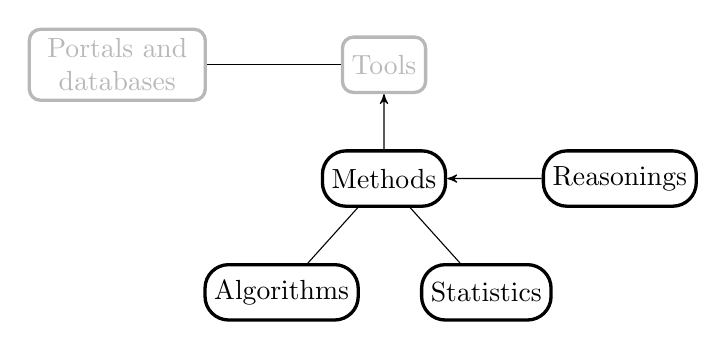
\begin{tikzpicture}[node distance=1.2cm, auto,scale=6]
%\path[use as bounding box] (0.1,0);  %-2, -2.6
 %nodes
\onslide+<1-> {

 \node[punkt,text width=2cm,color=light-gray] (bd) {Portals and databases};
 \node[right=of bd,xshift=5mm,punkt,color=light-gray] (tools) {Tools};
 \draw[-] (tools) to (bd);

 \node[below=of tools,yshift=5mm,punkk] (methods) {Methods};
 \node[right=of methods,punkk] (razon) {Reasonings};

 \draw[<-] (tools) to (methods);
% \draw[<-] (tools) to (razon);
 \draw[<-] (methods) to (razon);

 \node[below=of methods,xshift=-13mm,yshift=5mm,punkk] (algo) {Algorithms};
 \node[below=of methods,xshift=13mm,yshift=5mm,punkk] (stats) {Statistics};
% \node[below=of razon,punkk,yshift=5mm,text width=2cm] (filog) {Evoluci�n/ Filogenia};

 \draw[-] (methods) to (algo);
 \draw[-] (methods) to (stats);
% \draw[-] (razon) to (filog);

 % \node [xshift=-0.86cm,yshift=-7.35cm] at (current page.south west)  {\scriptsize[Secci�n \ref{D-bbms-objetivos-detalles}, p.\ \pageref{D-bbms-objetivos-detalles}]};


}


% {\footnotesize

%  \onslide+<2-> {
% \node[below=of stats,yshift=-2mm,xshift=23mm,text width=1.82cm,punkk] (criteria) {Desarrollo criterios};
%  \node[left=of criteria,punkk,xshift=5mm,text width=2.4cm] (man)
%  {Documentaci�n: Manuales, Literatura} 
%  edge [->] (criteria); 

%  \node[left=of man,punkk,text width=1.5cm,xshift=5mm] (info) {B�squeda info}
% edge [<-] (man);

%  \node[below=of man,punkk,text width=1.7cm]
%  (act) {Actitudes/ Aptitudes}
%  edge[->] (criteria)
%  edge[->] (info);
 
%  % \onslide+<4->\draw[-] (act) to (criteria);
%  % \onslide+<4->\draw[-] (act) to (info);

%  \draw[.,bend left,color=light-gray] (info) to (bd);
%  \draw[.,color=light-gray] (criteria) to (algo);
%  \draw[.,color=light-gray] (criteria) to (stats);
%  \draw[.,color=light-gray] (criteria) to (razon);

% }
% }


% \onslide+<3-> {

% }
\end{tikzpicture}
\end{frame}


%%% What follows is coming from "modelos.tex"

\begin{frame}
\frametitle{Where do predictions come from?}
\begin{center}
\includegraphics[%
     width=10.95cm,
     keepaspectratio]
{aemet.png}
\end{center}
\end{frame}


\begin{frame}
\frametitle{And these?}
\begin{center}
\includegraphics[%
     width=10.1cm,
     keepaspectratio]
{recession.png}
\end{center}
\end{frame}


\begin{frame}
\frametitle{Model according to the RAE}
\begin{center}
\includegraphics[%
     width=11.2cm,
     keepaspectratio]
{modelo-rae.png}
\end{center}
\end{frame}


\begin{frame}
\frametitle{Wikipedia}
\begin{center}
\includegraphics[%
     width=11.2cm,
     keepaspectratio]
{model-wikipedia.png}
\end{center}
\end{frame}


\begin{frame}
\frametitle{Wikipedia}
\begin{center}
\includegraphics[%
     width=11.2cm,
     keepaspectratio]
{model-wikipedia-2.png}
\end{center}
\end{frame}


\begin{frame}
  \frametitle{Models in biology}
  \begin{itemize}
  \item Lotka-Volterra
  \item Mendel's laws
  \item DNA replication and Okazaki fragments
\item Metabolic networks
\item Models of aminoacid and nucleotide substitution over time (evolution)
\item Models to predict 3D protein structure
\item etc.
  \end{itemize}
\end{frame}


\begin{frame}
  \frametitle{Models\   \ldots  models everywhere}
  \begin{itemize}
\item Models are everywhere!
\item We use them constantly in our daily life
\begin{itemize}
\item \textit{Driving}: model of a car, physics
\item \textit{Running, skiing, climbing}: model of a body, terrain, and physics
\item \textit{Dating}: model of human behavior and desires
\item \textit{Operating a stappler or a computer}: model of the machine
\item \ldots

\vspace*{15pt}
{\footnotesize (The idea of using a model is clearly present if you reason or think about
any of the above processes ---possibly different when no thinking
involved)}

\end{itemize}

\end{itemize}
\end{frame}




\begin{frame}
  \frametitle{Using the wrong model?}
\begin{center}
\includegraphics[%
     width=5.9cm,
     keepaspectratio]
{duty_calls.png}
\end{center}

  {\scriptsize From \Burl{http://xkcd.com/386/}}

\end{frame}



\begin{frame}
  \frametitle{A series of models}
  \begin{itemize}
  \item  $\uparrow \mbox{gene XYZ} \Rightarrow \uparrow P(\mbox{heart attack})$
\vspace*{10pt}
\pause
  \item $\uparrow \mbox{gene XYZ} \Rightarrow \uparrow P(\mbox{heart attack})$, \\
    $\uparrow \mbox{eating fish} \Rightarrow \downarrow P(\mbox{heart attack})$ 

\vspace*{10pt}

\pause
  \item $\uparrow \mbox{gene XYZ} \Rightarrow \uparrow P(\mbox{heart attack})$, \\
    $\uparrow \mbox{eating fish} \Rightarrow \downarrow P(\mbox{heart attack})$ \\
    $\uparrow \mbox{aerobic exercise} \Rightarrow \downarrow P(\mbox{heart attack})$ 


\vspace*{10pt}
\pause
\item $P(\mbox{heart attack}) = 0.003 + 0.9\ \mbox{gene XYZ} - 1\
  \mbox{tuna fish (kg.)} - 2\ \mbox{aerob.\ exer.\ (h.)} $

\vspace*{10pt}
\pause
\item $P(\mbox{heart attack}) = \alpha + \beta_1\ \mbox{gene XYZ} -
  \beta_2\  \mbox{tuna fish (kg.)} - \beta_3\ \mbox{aerob.\ exer.\ (h.)}$

where $\alpha = 0.003, \beta_1 = 0.9, \beta_2 = 1, \beta_3 = 2 $


\vspace*{4pt}
{\footnotesize And how do we find the $\beta$s?}
  \end{itemize}
\end{frame}



\begin{frame}
  \frametitle{Refining models}
  \begin{itemize}
  \item Verbal to quantitative
    \begin{itemize}
      \item Quantitative predictions
      \item Testable predictions
      \item Analyzing deviations from the model
    \end{itemize}

  \item Structure of the model. E.g., sums vs.\ products: additive effects
    vs.\ synergistic effects.
    \begin{itemize}
    \item Is the model appropriate?
    \end{itemize}

  \end{itemize}
\end{frame}




\begin{frame}
  \frametitle{What are they good for?}
  \begin{itemize}
  \item Predict
  \item Understand

\vspace*{15pt}

\item Does the model attempt to reflect true causal relationships? Purely
  phenomenological and ``working map''? Does this matter?
  \end{itemize}
\end{frame}



% \begin{frame}
%   \frametitle{Models with hidden variables and HMMs}
%   \begin{itemize}
%   \item Clustering
%   \item E.g.: clustering in breast cancer.
%   \end{itemize}
% \end{frame}


% \begin{frame}
%   \frametitle{HMMs}
% They are everywhere (ej., Krogh, Higgs and Attwood). Another two examples:
% \end{frame}



% \begin{frame}
% \begin{center}
% \includegraphics[%
%     width=11.0cm,
%     keepaspectratio]{hmm-1.png}
% \end{center}

% {\small (Remmert et al., 2012, \textit{Nature methods}, 9: 173--178)}

% \end{frame}


% \begin{frame}
% \begin{center}
% \includegraphics[%
%     width=11.2cm,
%     keepaspectratio]{hmm-2.png}
% \end{center}
% {\small (Ernst et al., 2011, \textit{Nature}, 473: 43--49)}

% \end{frame}




% \begin{frame}
%   \frametitle{HMMs}
%   \begin{itemize}
%   \item Quantitative
%   \item Structure
%   \end{itemize}
% \end{frame}



% \begin{frame}
%   \frametitle{HMM structure: not suited to other problems}
%   \begin{itemize}
%   \item RNAs
%   \end{itemize}
% \end{frame}


% \begin{frame}
%   \frametitle{Where do models live?}

% \vspace*{4cm}
% \centerline {\scriptsize Somewhere near where 2 + 2, or your idea of your
%   brother live}
% \end{frame}



\begin{frame}
  \frametitle{Recipes and algorithms}
We will need to ``do things'' with the data, follow a procedure, and get
answers: 

  \begin{itemize}
  \item {\LARGE \textbf{Algorithms}}

  
\item For example: $P(\mbox{heart attack}) = \alpha + \beta_1\ \mbox{gene
    XYZ} - \beta_2\ \mbox{kg.~ tuna fish} - \beta_3\ \mbox{h.~ aerob.\
    exer.}$
  
  where $\alpha = 0.003, \beta_1 = 0.9, \beta_2 = 1, \beta_3 = 2 $


  \vspace*{2pt}
  How do we find the $\beta$s?


\item We have been taught lots of algorithms over time (e.g., how to find
  a square root by hand). Algorithms, like models, are everywhere. 

  \end{itemize}

\end{frame}

\begin{frame}
  \frametitle{Algorithms}
\begin{itemize}
\item A very fast intro in Bloque I.

\item There are correct and incorrect algorithms. 

\item There are fast and slow
  (and memory hungry and memory efficient) algorithms. These things
  \textbf{do matter}, especially with real and large data.

\item A good algorithm might turn an unfeasible (or unsolvable) problem
  into something doable.

  \end{itemize}

\end{frame}


\section{BM-13: major topics}
\subsection{} %% to get the dots in header

\begin{frame}
  \frametitle{BM-13: Models, algorithms, and legos}
  \begin{itemize}
  \item Tools that are used in many different contexts
  \item Key: recognize similar structure
  \item Key: recognize an approach to solving the problem
  \item DP (dynamic programming), HMMs, etc.
  \end{itemize}
\end{frame}



\begin{frame}
  \frametitle{Seminars and invited classes}
  \begin{itemize}
  \item Intro talk by A.\ Valencia
  \item ENCODE: acess to data (note: this is wrong in the guia docente!)
  \item GENCODE and alternative splicing
  \item Functional genomics and evolution
%  \item Noise in gene expression
  \end{itemize}
\end{frame}




\begin{frame}
  \frametitle{Algorithms and probability}
  \begin{itemize}
  \item The basic building blocks
  \end{itemize}
\end{frame}


\begin{frame}
  \frametitle{Dynamic programming (DP), BLAST, alignment}
  
  \begin{itemize}
  \item Alignment is \ldots alignment. \textbf{Key in bioinformatics}
  \item Great first example
    \begin{itemize}
    \item Algorithms: from brilliant exact algorithms to heuristic algorithms
    \item And DP is \textbf{the} algorithm for many different problems
    \item Without probability: what can we say about solutions?
    \end{itemize}
  \end{itemize}
\end{frame}



\begin{frame}
  \frametitle{HMMs}

  \begin{itemize}
  \item A general purpose approach for \textbf{many different problems}
    (protein structure, gene prediction, segmentation, \ldots)
  \item Great second example
    \begin{itemize}
    \item Explicitly probabilistic
    \item A (family of) models
    \item Different algorithms: some DP
    \end{itemize}
  \end{itemize}
\end{frame}



\begin{frame}
  \frametitle{Phylogenetic reconstruction}
  \begin{itemize}
  \item Alignment (BLOSUM, PAM), similarities, etc: evolutionary arguments
  \item Recurrent themes
    \begin{itemize}
    \item Algorithms (and ``just algorithms'': NJ)
    \item Explicitly probabilistic models: how much do we want to assume?
    \end{itemize}
  \item And you get ready for ``Functional genomics and evolution''
  \end{itemize}
\end{frame}



\begin{frame}
  \frametitle{Statistics for omics}
  \begin{itemize}
  \item Make explicit a theme: differentiate ``true'' findings from
    ``capitalizing on chance''.
  \item Usim omics data to classify patients/diagnostics, etc:
    classification. 
  \item {\footnotesize (We will see few algorithms here)}
  \end{itemize}
\end{frame}


\begin{frame}
  \frametitle{Network reconstruction}
  \begin{itemize}
  \item ``Things are connected'': networks of relationships
    \begin{itemize}
    \item How do we infer structure?
    \item Algorithms. 
    \item And what is the probability of recovering true structure?
    \item Difference between structure learning and analysis.
    \end{itemize}
  \end{itemize}
\end{frame}




\begin{frame}
  \frametitle{What and why}
  \begin{itemize}
  \item Unrolling previous slides in reverse \ldots
  \end{itemize}
\end{frame}


\begin{frame}
  \frametitle{What will not be covered?}
  \begin{itemize}
  \item If we only cover a few things \ldots 
  \item we will not cover most of what falls under ``Bioinformatics''.

\pause
\vspace*{15pt}
\item Protein prediction and folding.
\item RNA prediction.
\item Sequencing (NGS and all that).
\item aCGH.
\item \ldots
  \end{itemize}
\end{frame}


\begin{frame}
  \frametitle{What will be covered?}
  \begin{itemize}
  \item Just a few things.
  \item We can argue all/most/many of them are of fundamental importance.
  \item Some are covered because of their general applicability and/or
    because they show a way of thinking about, and solving, problems.
  \end{itemize}
\end{frame}


\begin{frame}
\frametitle{Objectives: skills and attitudes}
\begin{itemize}
\item Acquire skills and attitudes
  \begin{itemize}
  \item Get used to reading and \textbf{working through} the primary literature
  \end{itemize}
\end{itemize}
\end{frame}




\section{Managing PDFs}
\subsection{} %% to get the dots in header


\begin{frame}
\frametitle{PDFs: reading, annotating, etc}
We want to avoid printing papers and moving around books.

\begin{itemize}
\item Linux: okular, evince.
\item Windows: PDF-XChange viewer
\item Mac: Papers?
\item Mendeley (\Burl{http://www.mendeley.com})
\item Zotero (\Burl{http://www.zotero.org})
\item Others: 
  \begin{itemize}
    \item  \Burl{http://www.bioinformatics.org/librarian}% (Note the poll results: what is the most asked for feature?)
    \item  \Burl{http://Docear.org}
    \item \Burl{http://readcube.com}
    \item \Burl{http://paperpile.com}
  \end{itemize}

\item E-readers?
\item Tablets?
\Burl{http://ligarto.org/rdiaz/Zotero-Mendeley-Tablet.html}
\item Searching a collection of pdfs.

\item And then, there is text mining. 

\end{itemize}
\end{frame}







\end{document}




%% Email
A.USO DE PORTATILES DEL AULA

El aula cuenta con 20 port�tiles macbook con dual boot (win y mac). Si los
usais, sereis responsables de sacarlos del armario y, al final de clase,
devolverlos al armario _Y_ dejarlos enchufados. (Esto lo repetiremos el
primer d�a que vayais a usar port�tiles).

B. USO DE VUESTROS PROPIOS PORTATILES

Por otra parte, si quereis, en vez de usar los port�tiles del departamento
podeis traer vuestros propios port�tiles. En ese caso deber�ais:

1. Configurar el acceso a la red inal�mbrica de la UAM, si a�n no lo
hab�is hecho. 

Instrucciones aqu�: http://www.uam.es/wifi

2. Tener un navegador (web browser) con los plugins de Java. 

Java se descarga de la p�gina de Sun: www.sun.com. Podeis verificar que
funciona visitando la p�gina 

http://3dsim.bioinfo.cnio.es

y seleccionando uno de los ejemplos. Deber�ais ver una prote�na, ser
capaces de marcar dominios, etc.

3. Tener Python instalado.

Una versi�n aceptablemente reciente (>= 2.5) basta. Pero es importante que
est� bastante completa, e incluya en particular el uso de Tcl/Tk. Podeis
verificar esto �ltimo siguiendo las instrucciones de Tkinter 
http://wiki.python.org/moin/TkInter

Basta con que llegueis con �xito a la Step 3. Todo lo dem�s (y qu� es
Tkinter) podeis ignorarlo.

4. Tener Pymol instalado. Lo m�s expeditivo es que useis una de las
versiones obsoletas pero pre-compiladas:

http://sourceforge.net/projects/pymol/files/Legacy/

(para los mac, el macpymol parece OK).



%%% Local Variables:
%%% ispell-local-dictionary: "en_US"
%%% coding: iso-8859-15
%%% TeX-master: t
%%% End:


